% preamble
% report --> small books, reports, etc...
\documentclass{report}
% used to show subsubsections in the table of contents.
\setcounter{tocdepth}{4}
\setcounter{secnumdepth}{4}

% needed if we want to put images
\usepackage{graphicx}

% used to make the table of contents clickable
\usepackage{hyperref}
\hypersetup{
    colorlinks,
    citecolor=black,
    filecolor=black,
    linkcolor=black,
    urlcolor=black
}

%used to make tables
\usepackage{booktabs}

% let's change this ugly serif font!
\renewcommand{\familydefault}{\sfdefault}

% used to manage images
\usepackage{float}

% now start with the RASD document
\begin{document}

\title{\textbf{myTaxiService} \\ -  \\ \textbf{Requirements Analysis and Specification Document}}
\author{Davide Cremona, Simone Deola}
\maketitle

\tableofcontents

\chapter{Introduction}

	\section{Purpose}
	This document is the R.A.S.D. (Requirement Analysis and Specification Document).
	The purpose of this document is the description of the "myTaxiService" system. 
	At first, it will provide functional and non-functional requirements, a complete overview of the constraints of the system and its limits. Then it will explain in detail the dynamics of the system using real-life use cases.
	Finally this document will provide a base for the developers that concretely have to implement the system.

	\section{Actual System}
	The functionality that the new system will provide is now not supported. 
	So the entire system must be developed without using or modifying existing system.

	\section{Scope}
	The objective of “myTaxiService” is to provide an interface between \hyperref[sec:customer]{customers} and \hyperref[sec:tdriver]{taxi drivers} to optimize their interaction and provide a fair management of taxi queues. The \hyperref[sec:normaluser]{users}, once registered through the mobile application or the web application, can request a taxi for their travel or reserve one, specifying the origin and the destination. The reservation can be done at least two hour before the ride; if the reservation can take place, the system will allocate a taxi 10 minutes before the meeting time.
	On the other side, \hyperref[sec:tdriver]{taxi drivers} can inform the system that they are waiting for a client and accept or decline a ride request. If the request has been accepted, a notification will be sent to the requesting \hyperref[sec:customer]{customer} with the identification number of the incoming taxi and the time he has to wait. Otherwise, if the request has been rejected it will be forwarded to the next taxi in the queue.
	The system has to optimize the management of \hyperref[sec:customer]{customers} requests giving the rides to the taxi with the highest priority that has to be evaluated in function of avaiability and the nearness of the \hyperref[sec:tdriver]{taxi driver}.

	\section{Actors}
		\begin{itemize}
		  \item \textbf{Guest User:}\label{sec:normaluser} guest users are unlogged or unregistered users. They can visit the login page or the registration forms.

		  \item \textbf{Registered User:}\label{sec:ruser} this kind of user identify either a Guest User or a Taxi Driver.

		  \item \textbf{Customer:}\label{sec:customer} this kind of user is the end-user of the service. He can perform request for taxis or reserve a ride. In his personal page he can view his requests and the system responses.

		  \item \textbf{Taxi Driver:}\label{sec:tdriver} this kind of user is composed by the actual taxi drivers that can only see customers requests that has been forwarded by the system. He can accept or decline these requests. Also, he's considered a special kind of user because one can register as a "Taxi Driver" only if he provide a valid Taxi licence.
		\end{itemize}

	\section{Goals}

		\begin{itemize}
			\item \textbf{\lbrack G.1\rbrack}\label{sec:g1} Allow \hyperref[sec:normaluser]{guest user} to become a \hyperref[sec:customer]{customer} creating a myTaxiService Account.

			\item \textbf{\lbrack G.2\rbrack}\label{sec:g2} Allow \hyperref[sec:normaluser]{guest user} to become a \hyperref[sec:customer]{customer} using his Facebook Account.

			\item \textbf{\lbrack G.3\rbrack}\label{sec:g3} Allow \hyperref[sec:normaluser]{guest user} to become a \hyperref[sec:tdriver]{taxi driver}.

			\item \textbf{\lbrack G.4\rbrack}\label{sec:g4} Allow \hyperref[sec:ruser]{registered user} to log in with myTaxiService account.

			\item \textbf{\lbrack G.5\rbrack}\label{sec:g5} Allow a \hyperref[sec:normaluser]{Registered User} to view or modify his username and email.

			\item \textbf{\lbrack G.6\rbrack}\label{sec:g6} Allow a \hyperref[sec:normaluser]{Registered User} to retrieve his password if he doesn't remember it.

			\item \textbf{\lbrack G.7\rbrack}\label{sec:g7} Allow a \hyperref[sec:normaluser]{RegisteredUser} to signal another one if he has made a bad use of the system.

			\item \textbf{\lbrack G.8\rbrack}\label{sec:g8} Allow \hyperref[sec:customer]{customer} to log in with Facebook account.

			\item \textbf{\lbrack G.9\rbrack}\label{sec:g9} Allow \hyperref[sec:customer]{customers} to require a taxi.

			\item \textbf{\lbrack G.10\rbrack}\label{sec:g10} Allow \hyperref[sec:customer]{customers} to reserve a ride.

			\item \textbf{\lbrack G.11\rbrack}\label{sec:g11} Allow \hyperref[sec:customer]{customers} to delete a previous reservations.

			\item \textbf{\lbrack G.12\rbrack}\label{sec:g12} Allow \hyperref[sec:tdriver]{taxi drivers} to accept or decline a ride request.

			\item \textbf{\lbrack G.13\rbrack}\label{sec:g13} Allow \hyperref[sec:tdriver]{taxi drivers} to notify their availability.
		\end{itemize}
		
	\section{Definitions, Acronyms, Abbreviations}
		
		\subsection{Definitions}

		\subsection{Acronyms}
			\begin{itemize}
				\item RASD: Requirement Analysis and Specification Documents.
				\item DD: Design Document.
				\item UML: Unified Modeling Language.
				\item OS: Operative System.
				\item API: Application Program Interface.
				\item GPS: Global Positioning System.
				\item HTTP: Hypertext Transfer Protocol.
				\item HTTPS: Secure Hypertext Transfer Protocol.
			\end{itemize}

		\subsection{Abbreviations}
			\begin{itemize}
				\item G.x is the x-Goal
				\item Req.x is the x-Functional Requirement
				\item Dom.x is the x-Domain Assumption
			\end{itemize}
		
	\section{Reference documents}
		\begin{itemize}
			\item \href{http://www.math.uaa.alaska.edu/~afkjm/cs401/IEEE830.pdf}{(IEE830) IEEE Recommended Practice for Software Requirements Specifications}
		\end{itemize}
		
	\section{Document overview.}
	Until now, we have given a general explanation about the software functionalities and a brief description about this document. Now we will describe what the rest of this RASD contains.\\
	In Section 2 we will focus more about system constraints and assumptions.\\
	In Section 3 we will describe requirements, typical scenarios and use-cases. In this section there is also a collection of UML diagrams that describes in particular the functionalities of the system.\\
	//TODO SECTION 4
		
\chapter{Overall Description}
	
	\section{Product perspective}
	The system will be composed of a web application and a mobile application developed for the three major OS ( Apple iOS, Android, Windows 10). The system will provide some API with the purpose of a future connection with another travel planning systems. 
		
	\section{User Characteristics}
	% this user here is ok and don't have to be hyperreferred
	The users that we suppose will use our system are of two types. the ones who want to find a taxi for a travel in the simplest way (\hyperref[sec:customer]{customers}). The others are \hyperref[sec:tdriver]{taxi drivers} that want to increment their productivity. The first ones must be able to access to a web browser or download and using a mobile application, the second ones also must have a taxi license.
		
	\section{Constrains}
		
		\subsection{Regulatory Policies}
		myTaxiService  has to meet regulatory policies about taxies in the countries where it will be used.

		\subsection{Hardware Limitations}
		The only hardware limitation that the myTaxiService mobile application has to meet will be the mobile phones characteristics. the rest of the system will be no affected by particular hardware limitations.

		\subsection{Software Limitations}
		myTaxiService mobile application has to be compatible with all major mobile operating systems (Android, Apple iOS, Windows 10).
		Also myTaxiService web application has to be compatible with all major browser (Chrome, Safari, Firefox, Microsoft Edge).

		\subsection{Parallel Operations}
		Our system must be able to perform parallel operations on the database to satisfy all the requests from multiple users.

		\subsection{Documents Related}

			\begin{itemize}
				\item Requirements and Analysis Specification Document (RASD)

				\item Design Document (DD)
			\end{itemize}

	\section{Assumptions}

			\begin{itemize}
				\item Every \hyperref[sec:tdriver]{taxi driver} has equipped a smartphone during working hours.

				\item Every \hyperref[sec:tdriver]{taxi driver} has a unique taxi license.

				\item Every taxi has a GPS locator to send GPS information to the central server.

				\item Android, Apple iOS or Windows 10 is avaiable on the \hyperref[sec:ruser]{registered users} smartphones.

				\item Every \hyperref[sec:ruser]{registered users} can be connected to the Internet with a mobile device when outside.

				\item When a \hyperref[sec:customer]{customer} require a taxi, the GPS informations about his location are automatically sended to the central server.

				\item The reservation of a ride is made at least two hours before the ride.

				\item Deletion of a reservation is made at least two hours before the ride.

				\item Requests from \hyperref[sec:customer]{customers} are automatically notified to the first \hyperref[sec:tdriver]{taxi driver} in the zone queue.

				\item If a \hyperref[sec:tdriver]{taxi driver} declines a request he will be placed in the bottom of the zone queue.

				\item If a request is declined it will be forwarded to the next \hyperref[sec:tdriver]{taxi driver} in the zone queue.

				\item If a \hyperref[sec:customer]{customer} make a bad use of the taxi request system, he can be reported as a bad \hyperref[sec:customer]{customer}.

				\item If a \hyperref[sec:tdriver]{taxi driver} notifies his availability is because he is actually avaiable

				\item If a \hyperref[sec:tdriver]{taxi driver} notifies his availability is because he wants to be notified of \hyperref[sec:customer]{customers} that needs a ride.

				\item If a \hyperref[sec:tdriver]{taxi driver} accept a request, the requesting \hyperref[sec:customer]{customer} will be notified
			\end{itemize}

	\section{Future possible Implementations}
	A possible future implementation can be a complex feedback system that permits to the \hyperref[sec:customer]{customers} to leave a comment about the \hyperref[sec:tdriver]{taxi driver} and vice versa.
	For example \hyperref[sec:tdriver]{taxi drivers} can be interested in knowing the punctuality or how is the behave of the \hyperref[sec:customer]{customer} that requests the ride.

\chapter{Specific Requirements}
This chapter contains a detailed description of how the applications works and its features. It also gives a specification of the functional and quality requirements.

	\section{External Interface Requirements}
	This section gives a description of the various inputs and relative outputs of the system. It also gives a description of the hardware, software and communication interfaces that are necessary to make the system work. It will also provide a generic visualization of the user interface in the various user platforms.

		\subsection{User Interfaces}
		Here we describe in particular how the application should look like either for mobile and web application. To make an easier explanation of the aspect of the various screen of 			the application we are going to use Mockup.
			\subsubsection{Login}
			On this page the users can log in with username and password or with Facebook (only if as registered user is a Customer). If the user is not already registered can access to the 					registration pages ( for Customer or for Taxi Drivers ). Also if the users forgot the password from this page can go to the forgot password page.
				
				\begin{figure}[H]
					\centering
					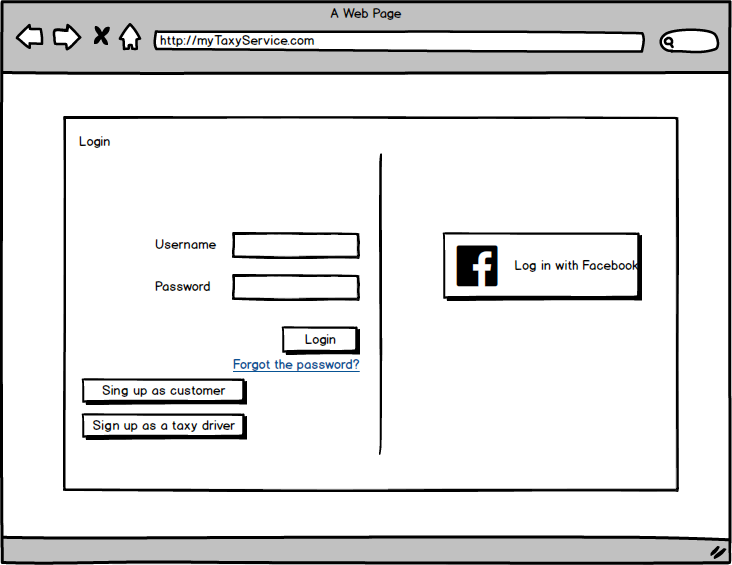
\includegraphics[scale=0.5]{IMG/UserInterfaces/CustomerLogin.png}
					\caption{Login Page, web version}\label{visina8}
				\end{figure}
				\begin{figure}[H]
					\centering
					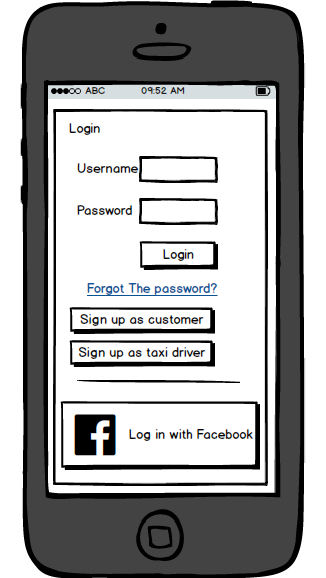
\includegraphics[scale=0.4]{IMG/UserInterfaces/CustomerLogin_m.png}
					\caption{Login Page, mobile version}\label{visina8}
				\end{figure}
			
			
			\subsubsection{Customer registration}
			On this page the users can register itself. This page must provide two way of registration, registration with the standard form ( e-mail, password and username) of with Facebook API.
			
				\begin{figure}[H]
					\centering
					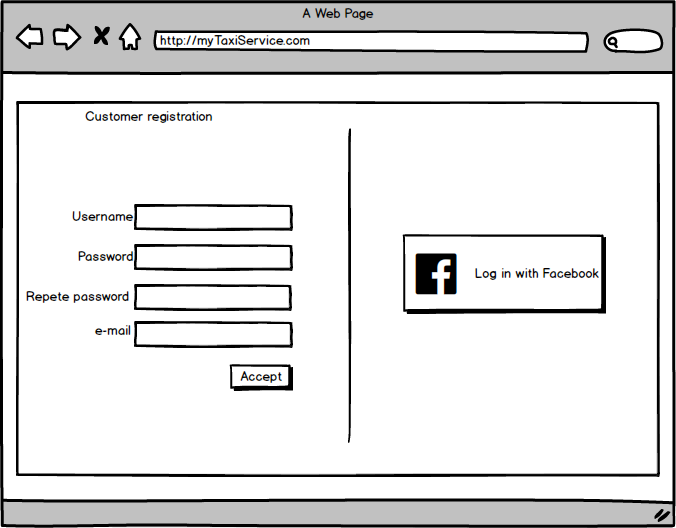
\includegraphics[scale=0.5]{IMG/UserInterfaces/CustomerRegistration.png}
					\caption{Customer registration Page, web version}\label{visina8}
				\end{figure}
				\begin{figure}[H]
					\centering
					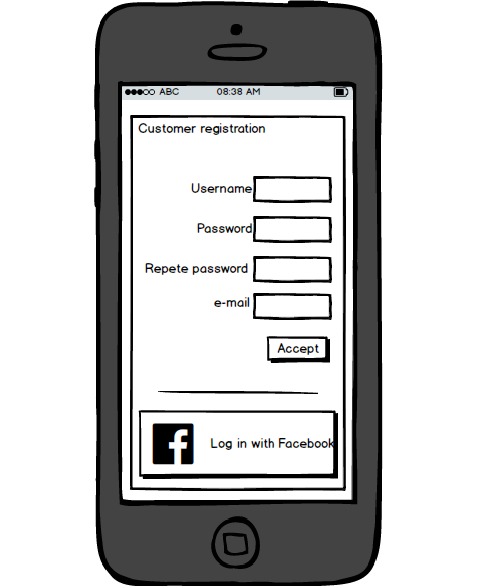
\includegraphics[scale=0.4]{IMG/UserInterfaces/CustomerRegistration_m.png}
					\caption{Customer registration Page, mobile version}\label{visina8}
				\end{figure}
			
			\subsubsection{Taxi Drivers registration}
			On this page the users can register itself as a taxi driver. Taxi driver have a special form to been registered because of the additional information the user must provide ( taxi license 				number). Just because the additional information the registration can be done just with the standard form.
				
				\begin{figure}[H]
					\centering
					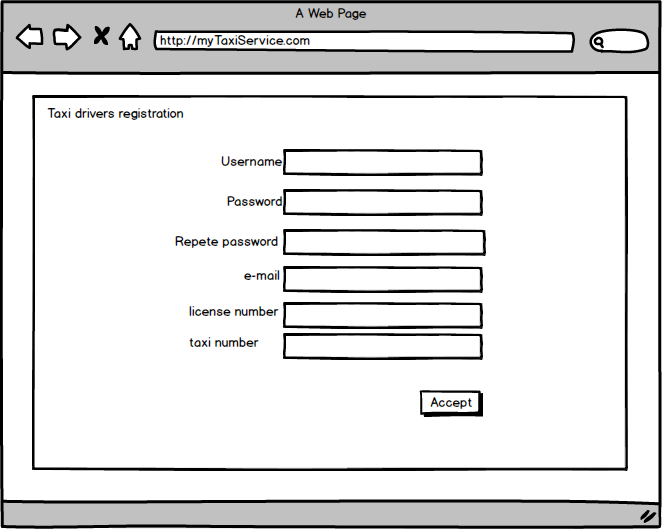
\includegraphics[scale=0.5]{IMG/UserInterfaces/TaxiDriverRegistration.png}
					\caption{Taxi Driver registration Page, web version}\label{visina8}
				\end{figure}
				\begin{figure}[H]
					\centering
					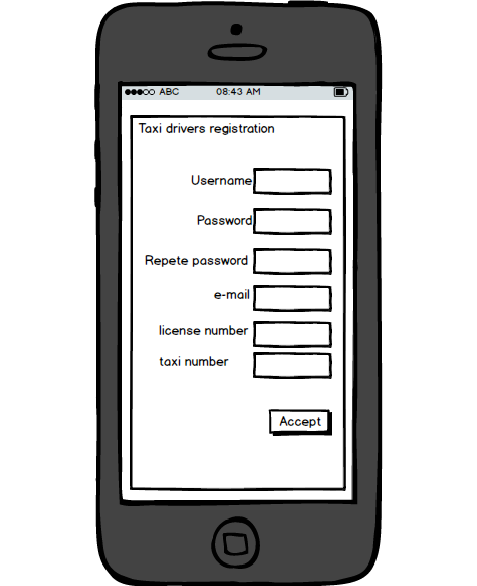
\includegraphics[scale=0.4]{IMG/UserInterfaces/TaxiDriverRegistration_m.png}
					\caption{Taxi Driver registration Page, mobile version}\label{visina8}
				\end{figure}
			
			\subsubsection{Customer home page}
			On this page the Customer can see his position (information from his GPS) and perform all the main operation that he can perform. He can Request a taxi on the position showed, can go to the reservation page (in which can reserve a ride), can visit his personal page (in which can see all the information of his profile), can go to the information page (information about myTaxiService) or go to the 'my reservation page' (in which can manage all the previous reserved ride). 
			
				\begin{figure}[H]
					\centering
					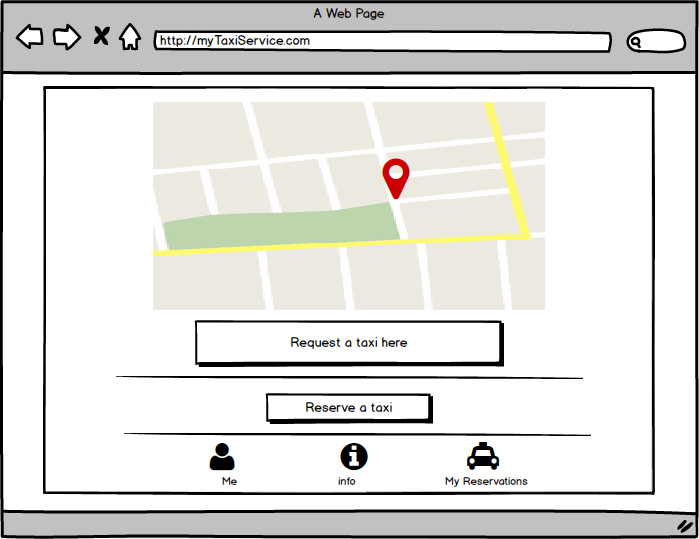
\includegraphics[scale=0.5]{IMG/UserInterfaces/mainCustomer.png}
					\caption{Customer home page, web version}\label{visina8}
				\end{figure}
				\begin{figure}[H]
					\centering
					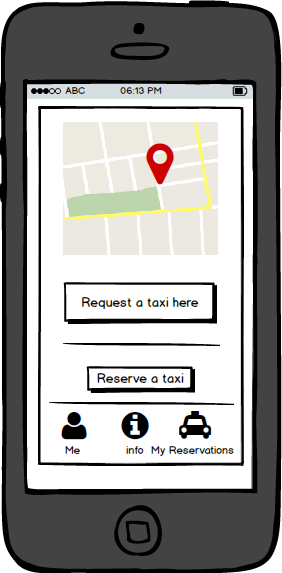
\includegraphics[scale=0.4]{IMG/UserInterfaces/mainCustomer_m.png}
					\caption{Customer home page, mobile version}\label{visina8}
				\end{figure}
			
			\subsubsection{Reservation page}
			On this page the Customer can reserve a taxi ride. To do this he mast insert a Origin position, a Destination position, a Data and a Time. The reservation must be at least two hours after 			the current Time, so the system must avoid to reserve a previous ride.
			
				\begin{figure}[H]
					\centering
					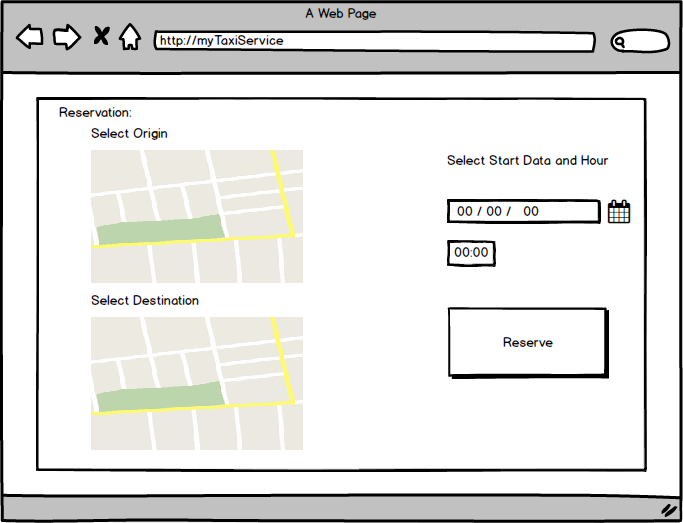
\includegraphics[scale=0.5]{IMG/UserInterfaces/reservationCustomer.png}
					\caption{Reservation page, web version}\label{visina8}
				\end{figure}
				\begin{figure}[H]
					\centering
					\includegraphics[scale=0.4]{IMG/UserInterfaces/reservationCustomer_m.png}
					\caption{Reservation page, mobile version}\label{visina8}
				\end{figure}
			
			\subsubsection{My reservation Page}
			On this page Customer can see all the reservation he have already done and adding some new. For each previous reservation can see all the information and, if the Date is before the 				next two hours, can delete it.			
			
				\begin{figure}[H]
					\centering
					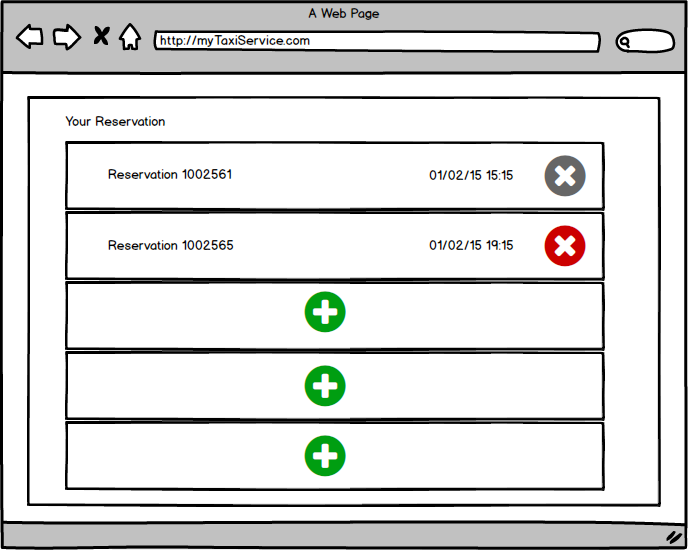
\includegraphics[scale=0.5]{IMG/UserInterfaces/myReservation.png}
					\caption{My reservation, web version}\label{visina8}
				\end{figure}
				\begin{figure}[H]
					\centering
					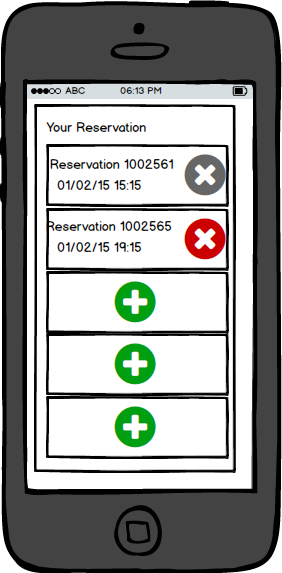
\includegraphics[scale=0.4]{IMG/UserInterfaces/myReservation_m.png}
					\caption{My reservation, mobile version}\label{visina8}
				\end{figure}
			
			
			\subsubsection{Customer notification pop-up}
			This pop-up is showed to the requesting Customer when his request has been handled. On this pop-up the system show also the number of the incoming taxi and an approssimative 				waiting time.
			
				\begin{figure}[H]
					\centering
					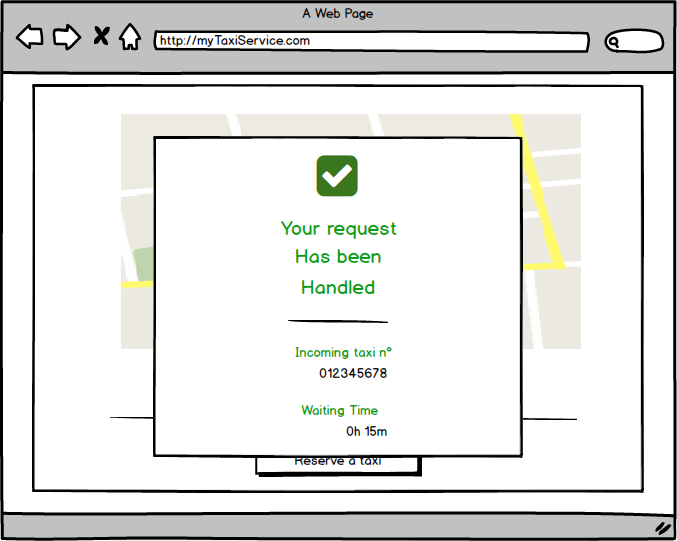
\includegraphics[scale=0.5]{IMG/UserInterfaces/customerNotification.png}
					\caption{Customer nofication, web version}\label{visina8}
				\end{figure}
				\begin{figure}[H]
					\centering
					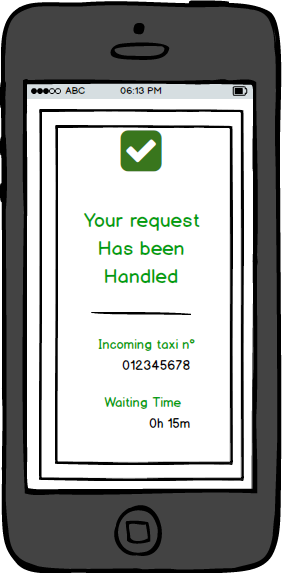
\includegraphics[scale=0.4]{IMG/UserInterfaces/customerNotification_m.png}
					\caption{Customer notification, mobile version}\label{visina8}
				\end{figure}
			
			\subsubsection{User page}
			This page show all the information about your user and show how many time you've been notified as bad user.
			
				\begin{figure}[H]
					\centering
					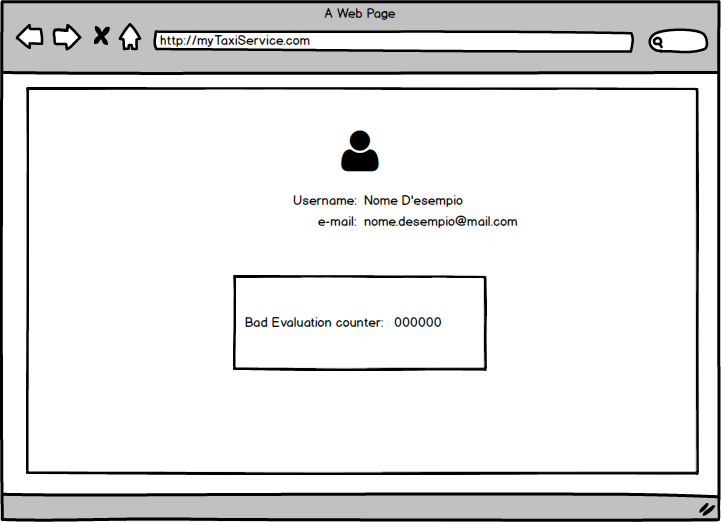
\includegraphics[scale=0.5]{IMG/UserInterfaces/userPage.png}
					\caption{User Page, web version}\label{visina8}
				\end{figure}
				\begin{figure}[H]
					\centering
					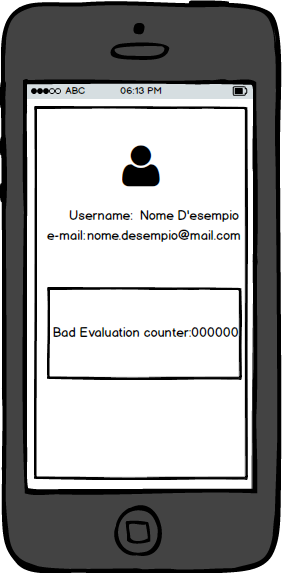
\includegraphics[scale=0.4]{IMG/UserInterfaces/userPage_m.png}
					\caption{User Page, mobile version}\label{visina8}
				\end{figure}

			
			\subsubsection{Taxi Driver home page}
			On this page the Taxi driver can see his position (information from his GPS) and inform the system about his availability.
			
				\begin{figure}[H]
					\centering
					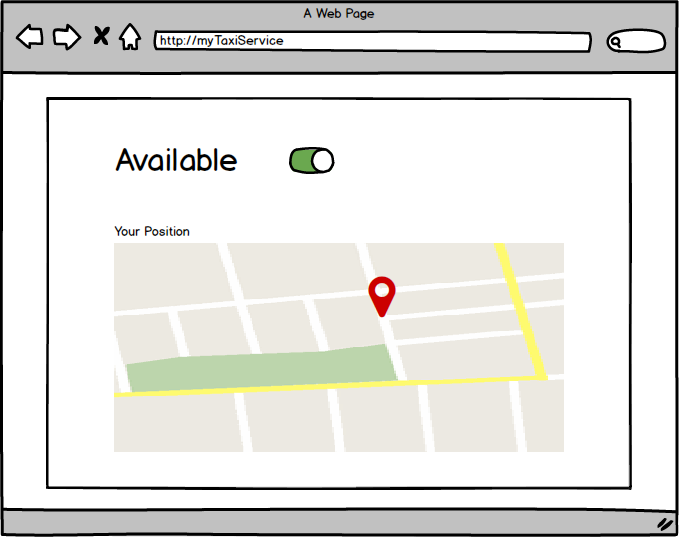
\includegraphics[scale=0.5]{IMG/UserInterfaces/mainTaxiDriver.png}
					\caption{Taxi driver home page, web version}\label{visina8}
				\end{figure}
				\begin{figure}[H]
					\centering
					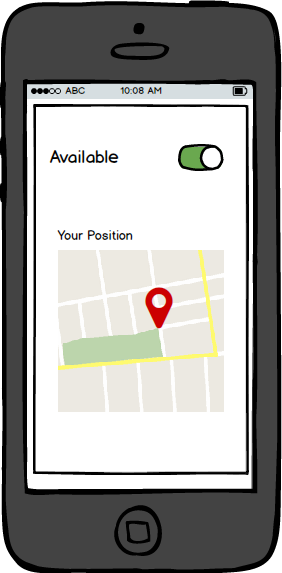
\includegraphics[scale=0.4]{IMG/UserInterfaces/mainTaxiDriver_m.png}
					\caption{Taxi driver home page, mobile version}\label{visina8}
				\end{figure}
			
			
			
			\subsubsection{Taxi Driver notification}
			On this pop-up the taxi driver will notified of a request that he can handle. On this pop-up is showed also two button, with which the taxi driver can accept or decline the request.
			
				\begin{figure}[H]
					\centering
					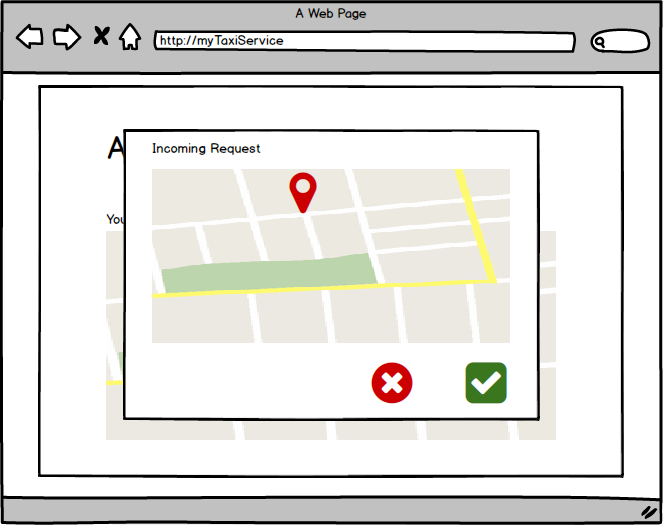
\includegraphics[scale=0.5]{IMG/UserInterfaces/notificationTaxiDriver.png}
					\caption{Taxi driver notification pop-up, web version}\label{visina8}
				\end{figure}
				\begin{figure}[H]
					\centering
					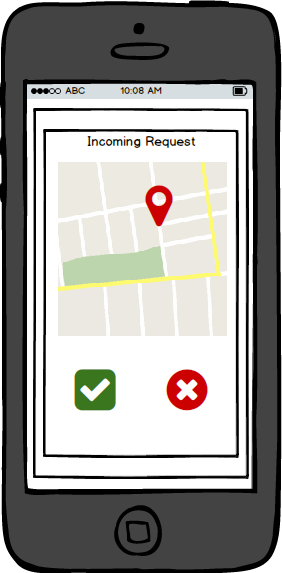
\includegraphics[scale=0.4]{IMG/UserInterfaces/notificationTaxiDriver_m.png}
					\caption{Taxi driver notification pop-up, mobile version}\label{visina8}
				\end{figure}
				
			
			\subsubsection{Taxi Driver end ride page}
			When a taxi driver accept a ride this page is showed up. On this page the taxi driver can check the name of the customer and the Origin position of his journey. When the ride is ended 				he can give a bad evaluation or simply end the ride and return to the main page.
				
				\begin{figure}[H]
					\centering
					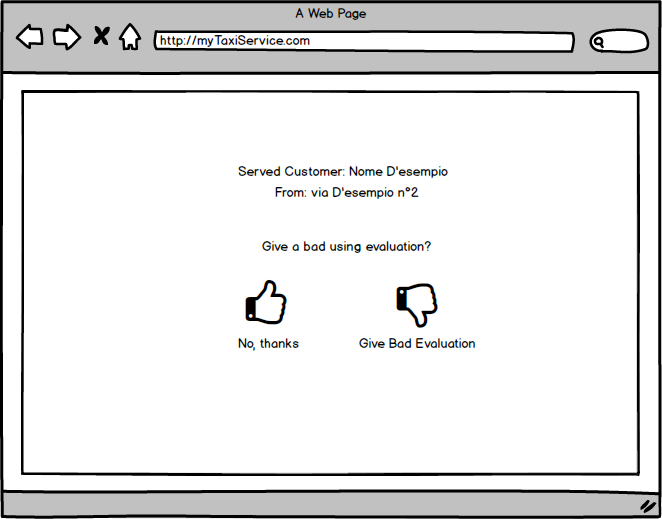
\includegraphics[scale=0.5]{IMG/UserInterfaces/onRidePage.png}
					\caption{On Ride Page, web version}\label{visina8}
				\end{figure}
				\begin{figure}[H]
					\centering
					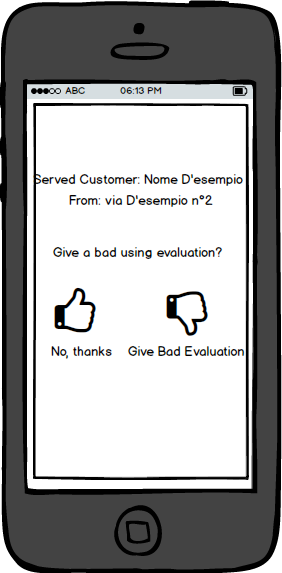
\includegraphics[scale=0.4]{IMG/UserInterfaces/onRidePage_m.png}
					\caption{On Ride page, mobile version}\label{visina8}
				\end{figure}
				

		\subsection{Hardware Interfaces}
		Since mobile and web applications don't have any dedicated hardware we have not designed any hardware interfaces for our system.
		The interaction with the central database is performed by connections handled by the already installed operating system on the mobile devices or the users computers.

		\subsection{Software Interfaces}
			\begin{itemize}
				\item The mobile application communicates with the GPS application in order to get geographical informations about the user.
				
				\item The web application communicates with the browser in order to get geographical informations about the user.
				
				\item Mobile and web applications communicates with the database through HTTP requests to the server.
			\end{itemize}

		\subsection{Interfaces to Others Application}
			\begin{itemize}
				\item myTaxiService web application require that at least one of these browsers is installed on the user Personal Computer:
			
					\begin{center}
						\begin{table}[h!]
							
							\begin{center}
								\caption{Browsers}
								\label{tab:browsersTable}

								\begin{tabular}{cccc}
									\toprule
									\textbf{Name} & \textbf{Version} & \textbf{Company} & \textbf{Source}\\
									\midrule
									Safari & 9.0.1 & Apple Inc. & \href{http://www.apple.com/safari/}{Get Safari}\\
									\midrule
									Firefox & 41.0 & Mozilla & \href{https://www.mozilla.org/en-US/firefox/new/}{Get Firefox}\\
									\midrule
									Chrome & 46.0.2490 & Google & \href{https://www.google.com/chrome/browser/desktop/}{Get Chrome}\\
									\midrule
									Microsofr Edge & 20.10240.16384.0 & Microsoft & \href{https://www.microsoft.com/en-us/download/details.aspx?id=48126}{Get Edge}\\
									\bottomrule
								\end{tabular}
							\end{center}
							
						\end{table}
					\end{center}

				\item myTaxiService mobile application require that at least one of these operating systems is installed on the user Smartphone:

					\begin{center}
						\begin{table}[h!]
							
							\begin{center}
								\caption{Mobile Operative Systems}
								\label{tab:mobileOSTable}

								\begin{tabular}{cccc}
									\toprule
									\textbf{Name} & \textbf{Version} & \textbf{Company} & \textbf{Source}\\
									\midrule
									Android & KitKat 4.4W.2 or later & Google & \href{https://www.android.com}{Android Info}\\
									\midrule
									iOS & 9.1 or later & Apple Inc. & \href{http://www.apple.com/ios/}{iOS Info}\\
									\midrule
									Windows 10 & 10.0.10572.0 or later & Microsoft & \href{http://www.microsoft.com/it-it/mobile/windows10/?dcmpid=omc-org-globalsite.globalredirect}{Windows 10 Info}\\
									\bottomrule
								\end{tabular}
							\end{center}
							
						\end{table}
					\end{center}

				\item To give an additional LogIn method, we use also the "LogIn with Facebook" API relased by Facebook. Facebook Login for Apps is a fast and convenient way for people to create accounts and log into our system across multiple platforms. It is well described at \href{https://developers.facebook.com/docs/facebook-login}{Facebook Login API Page.}
			\end{itemize}


		\subsection{Communication Interfaces}
		The communication between system pieces is not specified because it is handled by the underlying operating systems for both the mobile application and the web portal.

		In particular, the web and mobile applictaions will communicate with the server through HTTP/HTTPS requests. 

			\begin{itemize}
				\item HTTP communicate through the port number 80 and is handled by the operating system. 
				\item HTTPS communicate through the port number 443 and is handled by the operating system.
			\end{itemize}

	\section{Functional Requirements}
	In this section are described, for every Actor, the Functional Requirements needed to reach the linked Goal.

		\subsection{Functional Requirements for Guest Users}
		Here are listed all the Functional Requirements referring to the Goals that affects Guest Users.

			\subsubsection{\lbrack \hyperref[sec:g1]{G.1 - Allow guest users to become a customer creating a myTaxiService Account}\rbrack}
			To allow the guest user to perform a successful registration the system has to:

				\begin{itemize}
					\item \lbrack Req.1\rbrack \label{sec:fr1_g1} check if the selected username has not already been taken by another user to perform a successful registration.
					\item \lbrack Req.2\rbrack \label{sec:fr2_g1} check if the selected password is at least 8 characters long.
					\item \lbrack Req.3\rbrack \label{sec:fr3_g1} check if the selected password contains either digits and alphabetic characters.
					\item \lbrack Req.4\rbrack \label{sec:fr4_g1} check if the provided email has not already been used by another user.
					\item \lbrack Req.5\rbrack \label{sec:fr5_g1} check if the provided email respects this regular expression:\\ \textquotedblleft\textbackslash w+@\lbrack a-zA-Z\textunderscore\rbrack +?\textbackslash .\lbrack a-zA-Z\rbrack\textbraceleft2,3\textbraceright\textdollar\textquotedblright
					\item \lbrack Req.6\rbrack \label{sec:fr6_g1} ensures that the user cannot access to pages different from registration and login.
					\item \lbrack Req.7\rbrack \label{sec:fr7_g1} provide a registration page containing:
						\begin{enumerate}
							\item A text box where the user must insert his username.
							\item Two text box where the user must insert his password (the second one is for security check).
							\item A text box where the user must insert his email. 
							\item A button to submit informations to the system.
						\end{enumerate}
					\item \lbrack Dom.1\rbrack \label{sec:da1_g1} The email used by the Guest User is a valid one.
				\end{itemize}

			\subsubsection{\lbrack \hyperref[sec:g2]{G.2 - Allow guests user to become a customer using his Facebook Account}\rbrack}
			To allow the guest user to perform a successful registration using Facebook API, the system has to:

				\begin{itemize}
					\item \lbrack Req.1\rbrack \label{sec:fr1_g2} check if the Guest User is not already registered as a Customer.
					\item \lbrack Req.2\rbrack \label{sec:fr2_g2} delegate to the Facebook system all the checks concerning the existence of the user.
					\item \lbrack Req.3\rbrack \label{sec:fr3_g2} ensures that the user cannot access to pages different from registration and login.
 					\item \lbrack Req.4\rbrack \label{sec:fr4_g2} provide a registration page containing:
						\begin{enumerate}
							\item A button that calls the Facebook Registration API.
						\end{enumerate}
				\end{itemize}

			\subsubsection{\lbrack \hyperref[sec:g3]{G.3 Allow guest users to become a taxi driver}\rbrack}
			To allow the guest user to become a Taxi Driver, the system must:

			%"^\w+@[a-zA-Z_]+?\.[a-zA-Z]{2,3}$"

				\begin{itemize}
					\item \lbrack Req.1\rbrack \label{sec:fr1_g3} check if the selected username has not already been taken by another user.
					\item \lbrack Req.2\rbrack \label{sec:fr2_g3} check if the selected password is at least 8 character long.
					\item \lbrack Req.3\rbrack \label{sec:fr3_g3} check if the selected password contains either digits and alphabetic characters.
					\item \lbrack Req.4\rbrack \label{sec:fr4_g3} check if the provided email has not already ben used by another user.
					\item \lbrack Req.5\rbrack \label{sec:fr5_g3} check if the provided email respects this regular expression:\\ \textquotedblleft\textbackslash w+@\lbrack a-zA-Z\textunderscore\rbrack +?\textbackslash .\lbrack a-zA-Z\rbrack\textbraceleft2,3\textbraceright\textdollar\textquotedblright
					\item \lbrack Req.6\rbrack \label{sec:fr6_g3} ensures that the user cannot access to pages different from registration and login.
					\item \lbrack Req.7\rbrack \label{sec:fr7_g3} check if the provided taxi license has not already been used by another one.
					\item \lbrack Req.8\rbrack \label{sec:fr8_g3} provide a registration page containing:
						\begin{enumerate}
							\item A text box where the user must insert his username.
							\item Two text box where the user must insert his password (the second one is for security check).
							\item A text box where the user must insert his email.
							\item A text box where the user must insert his taxi license.
							\item A text box where the user must insert his taxi number.
							\item A button to submit informations to the system.
						\end{enumerate}
					\item \lbrack Dom.1\rbrack \label{sec:da1_g3} The email used by the Guest User is a valid one.
				\end{itemize}

		\subsection{Functional Requirements for Registered Users}

			\subsubsection{\lbrack \hyperref[sec:g4]{G.4 Allow registered users to log in with myTaxiService account.}\rbrack}
			To allow a registered user to log in with his myTaxiService account, the system must:

				\begin{itemize}
					\item \lbrack Req.1\rbrack \label{sec:fr1_g4} check if the given username is registered.
					\item \lbrack Req.2\rbrack \label{sec:fr2_g4} check if the given password is related to the given username.
					\item \lbrack Req.3\rbrack \label{sec:fr3_g4} ensures that the user cannot access to different pages from login and registration.
					\item \lbrack Req.4\rbrack \label{sec:fr4_g4} provide a login page containing:
						\begin{enumerate}
							\item A text box where the user must insert his username.
							\item A text box there the user must insert his password.
							\item A button to submit informations to the system.
						\end{enumerate}
				\end{itemize}

			\subsubsection{\lbrack \hyperref[sec:g5]{G.5 Allow a Registered User to view or modify his username and email.}\rbrack}
			To allow a Registered User to view or modify his username and email, the system must:

				\begin{itemize}
					\item \lbrack Req.1\rbrack \label{sec:fr1_g5} check if the Registered User is correctly logged in.
					\item \lbrack Req.2\rbrack \label{sec:fr2_g5} provide an homepage that contains:
						\begin{enumerate}
							\item A button that, if clicked, shows the page that contains the Registered User's informations.
						\end{enumerate}
					\item \lbrack Req.3\rbrack \label{sec:fr3_g5} provide a page used to show Registered User's informations that contains:
						\begin{enumerate}
							\item A clickable label showing the username of the Registered User.
							\item A clickable label showing the email of the Registered User.
							\item A box with a label inside that shows how many times the Registered User has been reported as a bad user.
						\end{enumerate}
					\item \lbrack Req.4\rbrack \label{sec:fr4_g5} once clicked, the username label must become a text box in wich the Registered User can write his new username. The system must also ensure that the new username is not already taken by another registered user. If it was taken, then the system will cancel the update. Otherwise the system will have to update the record in the database that refers to the registered user with the new username.
					\item \lbrack Req.5\rbrack \label{sec:fr5_g5} once clicked, the email label must become a text box in witch the Registered User can write his new email. The system must also ensure that the new email is not already taken by another registered user and respects the regular expression:\\ \textquotedblleft\textbackslash w+@\lbrack a-zA-Z\textunderscore\rbrack +?\textbackslash .\lbrack a-zA-Z\rbrack\textbraceleft2,3\textbraceright\textdollar\textquotedblright.\\ If it was taken, then the system will cancel the update. Otherwise the system will have to update the record in the database that refers to the registered user with the new username.
				\end{itemize}

			\subsubsection{\lbrack \hyperref[sec:g6]{G.6 Allow a Registered User to retrieve his password if he doesn't remember it.}\rbrack}
			To allow a Registered User to retrieve his password, the system must:

				\begin{itemize}
					\item \lbrack Req.1\rbrack \label{sec:fr1_g6} on the log in page, provide a link that will call the function of the system that will send an email to the Registered User with his password.
				\end{itemize}

			\subsubsection{\lbrack \hyperref[sec:g7]{G.7 Allow a Registered Users to signal another one if he has made a bad use of the system.}\rbrack}
			To allow a Registered User to signal another one, the system must:

				\begin{itemize}
					\item \lbrack Req.1\rbrack \label{sec:fr1_g7} check if the Registered User is correctly logged in.
					\item \lbrack Req.2\rbrack \label{sec:fr2_g7} for Taxi Drivers, provide an end-ride page that contains:
						\begin{enumerate}
							\item A label showing the username of the Customer that he has just served.
							\item A label showing the starting location of the current ride.
							\item A label that asks to the Taxi Driver if he want to report the Customer.
							\item A button that, if clicked, ends the current ride calling the function of the system that sets to \textquotedbleft ended\textquotedbright the current ride without reporting the Customer.
							\item A button that, if clicked, A button that, if clicked, ends the current ride calling the function of the system that sets to \textquotedbleft taxi-ended\textquotedbright the current ride and increments the Customer's Bad Evaluation Counter.
						\end{enumerate}
					\item \lbrack Req.3\rbrack \label{sec:fr3_g7} After that one of the Taxi Driver end-ride page button is pressed, the system must ensure that the page is not reachable anymore and the Taxi Driver must access only to his homepage.
					\\
					\item \lbrack Req.4\rbrack \label{sec:fr4_g7} for Customers, provide an end-ride page that contains:
						\begin{enumerate}
							\item A label showing the username of the Taxi Driver that has just served him.
							\item A label showing the starting location of the current ride.
							\item A label that asks to the Customer if he want to report the Taxi Driver.
							\item A button that, if clicked, ends the current ride calling the function of the system that sets to \textquotedbleft ended\textquotedbright the current ride without reporting the Taxi Driver.
							\item A button that, if clicked, ends the current ride calling the function of the system that sets to \textquotedbleft customer-ended\textquotedbright the current ride and increments the Taxi Driver's Bad Evaluation Counter.
						\end{enumerate}
					\item \lbrack Req.5\rbrack \label{sec:fr5_g7} After that one of the Customer end-ride page button is pressed, the system must ensure that the page is not reachable anymore and the Customer must access only to his homepage.
					\item \lbrack Dom.1\rbrack \label{sec:da1_g7} The ride is ended after a Taxi Driver or a Customer action.
				\end{itemize}

		\subsection{Functional Requirements for Customers}

			\subsubsection{\lbrack \hyperref[sec:g8]{G.8 Allow customers to log in with Facebook account.}\rbrack}
			To allow a customer to log in with Facebook account, the system must:

				\begin{itemize}
					\item \lbrack Req.1\rbrack \label{sec:fr1_g8} provide a button that calls the Facebook Login API.
					\item \lbrack Req.2\rbrack \label{sec:fr2_g8} delegate to the Facebook system all the checks about the existence of the user.
				\end{itemize}

			\subsubsection{\lbrack \hyperref[sec:g9]{G.9 Allow customers to require a taxi.}\rbrack}
			To allow the customers to require a taxi, the system must:

				\begin{itemize}
					\item \lbrack Req.1\rbrack \label{sec:fr1_g9} check if the customer is correctly logged in.
					\item \lbrack Req.2\rbrack \label{sec:fr2_g9} provide an homepage that contains:
						\begin{enumerate}
							\item A map showing the current location of the customer.
							\item A button that calls the function of the system to require a taxi (called "require button").
						\end{enumerate}
					\item \lbrack Req.3\rbrack \label{sec:fr3_g9} once the "require button"is clicked (or tapped) the system must memorize the request in the remote database.
					\item \lbrack Req.4\rbrack \label{sec:fr4_g9} once the request is memorized in the database, the system must send a request notification to the first Taxi Driver available on the zone queue.
					\item \lbrack Req.5\rbrack \label{sec:fr5_g9} once the request has been accepted by a Taxi Driver, the system must send a notification to the customer with the incoming taxi informations and the supposed waiting time.
				\end{itemize}

			\subsubsection{\lbrack \hyperref[sec:g10]{G.10 Allow customers to reserve a ride.}\rbrack}
			To allow the customers to reserve a ride, the system must:

				\begin{itemize}
					\item \lbrack Req.1\rbrack \label{sec:fr1_g10} check if the customer is correctly logged in.
					\item \lbrack Req.2\rbrack \label{sec:fr2_g10} provide an homepage that contains:
						\begin{enumerate}
							\item A button that, if clicked, shows the page used to reserve a ride.
						\end{enumerate}
					\item \lbrack Req.3\rbrack \label{sec:fr3_g10} provide a page used to reserve a ride that contains:
						\begin{enumerate}
							\item A map where the customer can select the starting location for his ride.
							\item A map where the customer can select the ending location for his ride.
							\item A field where the customer can insert the starting date for the ride.
							\item A field where the customer can insert the starting time for the ride.
							\item A button that calls the function of the system to reserve a ride (called "reserve button").
						\end{enumerate}
					\item \lbrack Req.4\rbrack \label{sec:fr4_g10} "reserve button" must be clickable if and only if the reserve date and time is at least two hours after the current time. (for instance: if the current date is 10/10/2015 and current time is 10.00, the reservation time must be at least 12.00 of the 10/10/2015).
					\item \lbrack Req.5\rbrack \label{sec:fr5_g10} after the "reserve button" is clicked (or tapped) the system must memorize the reservation in the remote database.
					\item \lbrack Req.6\rbrack \label{sec:fr6_g10} once the reservation is memorized, the system must send a request notification 10 minutes before the starting time of the ride to the first Taxi Driver available on the zone queue.
					\item \lbrack Req.7\rbrack \label{sec:fr7_g10} once the ride has been accepted by a Taxi Driver, the system must send a notification to the customer with the incoming taxi informations and the supposed waiting time.
				\end{itemize}

			\subsubsection{\lbrack \hyperref[sec:g11]{G.11 Allow customers to delete a previous reservations.}\rbrack}
			To allow a customer to delete a previous reservation, the system must:

				\begin{itemize}
					\item \lbrack Req.1\rbrack \label{sec:fr1_g11} check if the customer is correctly logged in.
					\item \lbrack Req.2\rbrack \label{sec:fr2_g11} provide an homepage that contains:
						\begin{enumerate}
							\item A button that, if clicked, shows the page that contains all the reservations made by the customer.
						\end{enumerate}
					\item \lbrack Req.3\rbrack \label{sec:fr3_g11} provide a page that contains all the reservations made by the customer:
						\begin{enumerate}
							\item All reservations that have a difference between the start time and the current time of less than two hours are not erasable
							\item Other reservations are erasable.
							\item The page also contains a button to add a new reservation. If clicked that button leads the customer to the page used to reserve a ride (described in the Functional Requirements \hyperref[sec:fr3_g4]{Req.3 of G.4})
						\end{enumerate}
					\item \lbrack Dom.1\rbrack \label{sec:da1_g11} The reservation is deleted after the Customer action.
				\end{itemize}

		\subsection{Functional Requirements for Taxi Drivers}

			\subsubsection{\lbrack \hyperref[sec:g12]{G.12 Allow Taxi Drivers to accept or decline a ride request.}\rbrack}
			To allow Taxi Drivers to accept or decline ride requests, the system must:

			%The Taxi Driver must be already registered and logged in with a myTaxiService account.

				\begin{itemize}
					\item \lbrack Req.1\rbrack \label{sec:fr1_g12} check if the Taxi Driver is correctly logged in.
					\item \lbrack Req.2\rbracl \label{sec:fr2_g12} check if the state of the Taxi Driver is: Available.
					\item \lbrack Req.2\rbrack \label{sec:fr3_g12} if the Taxi Driver is at the top of his zone queue, the system must notify him with a request notification as described in \hyperref[sec:fr4_g9]{Req.4 of G.9}.
					\item \lbrack Req.3\rbrack \label{sec:fr4_g12} once the notification has been sent, the system must wait for the Taxi Driver acceptance or declination for 10 minutes, after that time, the request is forwarded to the next Taxi Driver in the zone queue.
					\item \lbrack Req.4\rbrack \label{sec:fr5_g12} if the request has been accepted, the Taxi Driver must be redirected to the end-ride page where he can end the ride when he want. Also he is moved to the bottom of his zone queue and his state is setted to Not Available.
					\item \lbrack Req.3\rbrack \label{sec:fr6_g12} if the request has been rejected, the Taxi Driver must be moved at the bottom of the zone queue and the Customer request is forwarded to the next Taxi Driver in the zone queue. Also the Taxi Driver is redirected to his home page and his state is setted to Available.
				\end{itemize}


			\subsubsection{\lbrack \hyperref[sec:g13]{G.13 Allow Taxi Drivers to notify their availability.}\rbrack}

				\begin{itemize}
					\item \lbrack Req.1\rbrack \label{sec:fr1_g13} check if the Taxi Driver is correctly logged in.
					\item \lbrack Req.1\rbrack \label{sec:fr1_g13} provide an home page that contains:
						\begin{enumerate}
							\item An ON/OFF button that signals to the system that the Taxi Driver is Available/Not Available.
							\item A map showing his current zone and position.
						\end{enumerate}
				\end{itemize}


	\section{Scenarios}


	\section{UML Models}

		\subsection{Use-Case Diagrams}

		\subsection{Class Diagrams}

		\subsection{State Machine Diagrams}

	\section{Non Functional Requirements}

		\subsection{Performance Requirements}

		\subsection{Design Constraints}

		\subsection{Software System Attributes}

			\subsubsection{Availability}

			\subsubsection{Maintainability}

			\subsubsection{Portability}

		\subsection{Security}

			\subsubsection{External Interface Side}

			\subsubsection{Application Side}

			\subsubsection{Server Side}


\chapter{Appendix}
//TODO
\end{document}